\documentclass[ 12pt ]{article}

\usepackage{amsmath}
\usepackage{amssymb}
\usepackage{cancel}
\usepackage{tikz}
\usepackage{tkz-fct}
\usepackage{tkz-euclide}
\usepackage{pgfplots}

\begin{document}

% title page
\title{Homework 2}
\author{Landon Fox}
\date{February 5, 2020}

\begin{flushleft}
Landon Fox \\
MATH 295 \\
Section 1001 \\
February 5, 2020
\end{flushleft}
\begin{center}
Homework 2
\end{center}

% problem 1
\section{}

\def\firstcircle{(-1,1) circle (1.5cm)}
\def\secondcircle{(1,1) circle (1.5cm)}
\def\thirdcircle{(0,-1) circle (1.5cm)}
\def\rectangle{(-4,-3) rectangle (4,3)}

\colorlet{circle edge}{gray!50}
\colorlet{circle area}{black!20}

\tikzset{filled/.style={fill=circle area, draw=circle edge, thick},
    outline/.style={draw=circle edge, thick}}

% problem 1i
\subsection{}
\begin{flalign}
A \cap (B-C)
\end{flalign}

\setlength{\parskip}{5mm}
\begin{center}
\begin{tikzpicture}
    \begin{scope}
        \clip \firstcircle;
        \clip \secondcircle;
        \fill[filled] \secondcircle;
        \fill[white] \thirdcircle;
    \end{scope}
    \draw[outline] \rectangle;
    \draw[outline] \firstcircle node[above] {$A$};
    \draw[outline] \secondcircle node[above] {$B$};
    \draw[outline] \thirdcircle node[below] {$C$};
    \draw (4,3.5) node {$S$};
\end{tikzpicture}
\end{center}
\newpage

% problem 1ii
\subsection{}
\begin{flalign}
(A \cap B) \cup (A \cap C)
\end{flalign}

\setlength{\parskip}{5mm}
\begin{center}
\begin{tikzpicture}
    \begin{scope}
        \clip \firstcircle;
        \clip \secondcircle;
        \fill[filled] \secondcircle;
    \end{scope}
    \begin{scope}
        \clip \firstcircle;
        \clip \thirdcircle;
        \fill[filled] \thirdcircle;
    \end{scope}
    \draw[outline] \rectangle;
    \draw[outline] \firstcircle node[above] {$A$};
    \draw[outline] \secondcircle node[above] {$B$};
    \draw[outline] \thirdcircle node[below] {$C$};
    \draw (4,3.5) node {$S$};
\end{tikzpicture}
\end{center}
\newpage

% problem 1iii
\subsection{}
\begin{flalign}
(A \cap \overline{B}) \cup (A \cap \overline{C})
\end{flalign}

\setlength{\parskip}{5mm}
\begin{center}
\begin{tikzpicture}
    \begin{scope}
        \fill[filled] \firstcircle;
        \clip \firstcircle;
        \clip \secondcircle;
        \clip \thirdcircle;
        \fill[white] \thirdcircle;
    \end{scope}
    \draw[outline] \rectangle;
    \draw[outline] \firstcircle node[above] {$A$};
    \draw[outline] \secondcircle node[above] {$B$};
    \draw[outline] \thirdcircle node[below] {$C$};
    \draw (4,3.5) node {$S$};
\end{tikzpicture}
\end{center}
\newpage

% problem 2
\section{}
Show:
\begin{flalign}
(A - B) - C = (A - C) - (B - C)
\end{flalign}

\subsection{Truth Table}
\begin{center}
\begin{tabular}{ |c|c|c|c|c| } 
 \hline
 A & B & C & (A - B) - C & (A - C) - (B - C) \\ 
 F & F & F & F & F \\
 F & F & T & F & F \\
 F & T & F & F & F \\
 F & T & T & F & F \\
 T & F & F & T & T \\
 T & F & T & F & F \\
 T & T & F & F & F \\
 T & T & T & F & F \\
 \hline
\end{tabular}
\end{center}

\subsection{Identities}
Note:
\begin{flalign}
(A - B) &= A\cap \overline{B}
\end{flalign}
\begin{flalign}
(A - B) - C &= (A - C) - (B - C) \\
(A \cap \overline{B}) \cap \overline{C} &= (A \cap \overline{C}) \cap \overline{(B \cap \overline{C})} \\
A \cap \overline{B} \cap \overline{C} &= (A \cap \overline{C}) \cap (\overline{B} \cup C) \\
&= ( (A \cap \overline{C}) \cap \overline{B} ) \cup ( (A \cap \overline{C}) \cap C ) \\
&= ( A \cap \overline{C} \cap \overline{B} ) \cup ( A \cap (\overline{C} \cap C) ) \\
&= ( A \cap \overline{B} \cap \overline{C} ) \cup ( A \cap \phi ) \\
&= ( A \cap \overline{B} \cap \overline{C} ) \cup \phi \\
A \cap \overline{B} \cap \overline{C} &= A \cap \overline{B} \cap \overline{C}
\end{flalign}

% problem 3
\section{}
\begin{flalign}
[0,x]\times[0,\frac{1}{x}]
\end{flalign}

\begin{center}
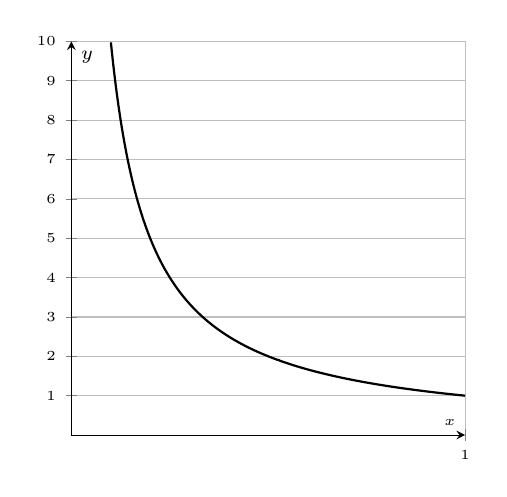
\begin{tikzpicture}
\begin{axis}%
    [
        grid=major,  
        x=50mm,
        y=5mm,
        xtick={0,1},   
        xmin=0,
        xmax=1,
        xlabel={\tiny $x$},
        axis x line=middle,
        ytick={0,...,10},
        tick label style={font=\tiny},
        ymin=0,
        ymax=10,
        ylabel={\scriptsize $y$},
        axis y line=middle,
        no markers,
        samples=100,
        domain=0:1,
        restrict y to domain=0:10
    ]
    \addplot[thick,samples=400] (x,{1/x});
    \addplot[dashed, samples=400] (x,{1/(x-2)});
\end{axis} 
\end{tikzpicture}
\end{center}

% problem 3i
\subsection{}
Find:
\begin{flalign}
\bigcap_{x\epsilon(0,1]}[0,x]\times[0,\frac{1}{x}] = \{\, (0,y):y\,\epsilon\,[0,1]\, \}
\end{flalign}

% problem 3ii
\subsection{}
Find:
\begin{flalign}
\bigcup_{x\epsilon(0,1]}[0,x]\times[0,\frac{1}{x}] = \{\, (x,y):0\leq y\leq \frac{1}{x}, x\,\epsilon\,[0,1]\, \}
\end{flalign}

% problem 4
\section{}

% problem 4i
\subsection{}
Prove or Disprove:
\begin{flalign}
A \cup C = B \cup C \rightarrow A=B
\end{flalign}
Counter-example:
\begin{flalign}
let\;\;\; A &= \{1,2\} \\
B &= \{1,2,3\} \\
C &= \{1,3\} \\
A\cup C &= \{1,2,3\} \\
B\cup C &= \{1,2,3\} \\
A &\neq B \\
\therefore A \cup C = B &\cup C \cancel{\rightarrow} A=B
\end{flalign}

% problem 4ii
\subsection{}
Prove or Disprove:
\begin{flalign}
A \cap C = B \cap C \rightarrow A=B
\end{flalign}
Counter-example:
\begin{flalign}
let\;\;\; A &= \{1,3\} \\
B &= \{1,2,3\} \\
C &= \{1,4\} \\
A\cap C &= \{1\} \\
B\cap C &= \{1\} \\
A &\neq B \\
\therefore A \cap C = B &\cap C \cancel{\rightarrow} A=B
\end{flalign}

% problem 5i
\section{}

\subsection{}
Note:
\begin{flalign}
A \Delta B = (A \cup B) - (A \cap B)
\end{flalign}
Determine if the symmetric difference is associative:
\begin{center}
\begin{tabular}{ |c|c|c|c|c|c|c| } 
 \hline
A & B & C & (B$\cup$ C)-(B$\cap$ C) & A $\Delta$ (B $\Delta$ C) & (A$\cup$ B)-(A$\cap$ B) & (A $\Delta$ B) $\Delta$ C \\ 
F & F & F & F & F & F & F \\
F & F & T & T & T & F & T \\
F & T & F & T & T & T & T \\
F & T & T & F & F & T & F \\
T & F & F & F & T & T & T \\
T & F & T & T & F & T & F \\
T & T & F & T & F & F & F \\
T & T & T & F & T & F & T \\
 \hline
\end{tabular}
\end{center}
Based off the truth table, the symmetric difference is associative due to the equivalence of the statements.
\newpage

% problem 5ii
\subsection{}
Prove or Disprove:
\begin{flalign}
A \Delta C = B \Delta C \rightarrow A=B
\end{flalign}
Note:
\begin{flalign}
A=B \rightarrow \forall x\{x\,\epsilon\,A\leftrightarrow\,x\epsilon\,B\}
\end{flalign}
Proof:
\begin{flalign}
assume\;\;\;&A \Delta C = B \Delta C \\
let\;\;\; &x\,\epsilon\, A \Delta C \\
if\;\;\; &x\,\epsilon\, A \\
know\;\;\; &x\,\epsilon\, A \wedge x\,\epsilon\, A \Delta C \rightarrow x\,\cancel{\epsilon}\, C \\
also\, know\;\;\; &x\,\epsilon\, A \Delta C \wedge A \Delta C = B \Delta C \rightarrow x\,\epsilon\, B \Delta C \\
&x\,\epsilon\, B \Delta C \wedge x\,\cancel{\epsilon}\, C \rightarrow x\,\epsilon\, B
\end{flalign}
\begin{flalign}
let\;\;\; &x\,\epsilon\, B \Delta C \\
if\;\;\; &x\,\epsilon\, B \\
know\;\;\; &x\,\epsilon\, B \wedge x\,\epsilon\, B \Delta C \rightarrow x\,\cancel{\epsilon}\, C \\
also\, know\;\;\; &x\,\epsilon\, B \Delta C \wedge B \Delta C = A \Delta C \rightarrow x\,\epsilon\, A \Delta C \\
&x\,\epsilon\, A \Delta C \wedge x\,\cancel{\epsilon}\, C \rightarrow x\,\epsilon\, A
\end{flalign}
\begin{flalign}
A \Delta C &= B \Delta C \rightarrow \forall x\{x\,\epsilon\,A\leftrightarrow\,x\epsilon\,B\} \\
\therefore A \Delta C &= B \Delta C \rightarrow A=B
\end{flalign}

\end{document}
